\documentclass[journal,12pt,onecolumn]{IEEEtran}
\usepackage{graphicx, float}
\graphicspath{{Figs/}}
\usepackage{multicol}
\usepackage{parskip}
\usepackage{titlesec}
\usepackage{color}
\usepackage{enumitem}
\usepackage{amsmath,amssymb,amsfonts,amsthm}
\usepackage{array}
\usepackage{booktabs}
\usepackage[table]{xcolor}
\usepackage{longtable}
\usepackage{gensymb}
\usepackage{cite}
\usepackage{algorithmic}
\usepackage{textcomp}
\usepackage{txfonts}
\usepackage{listings}
\usepackage{mathtools}
\usepackage{comment}
\usepackage{tkz-euclide}
\usepackage[breaklinks=true]{hyperref}
\usepackage{gvv}
\usepackage[utf8]{inputenc}
\usetikzlibrary{arrows.meta, positioning}
\usepackage{xparse}
\usepackage{calc}
\usepackage{multirow}
\usepackage{hhline}
\usepackage{ifthen}
\usepackage{lscape}
\usepackage{tabularx}

\begin{document}

\title{
ASSIGNMENT 1: GATE 2015 \\
BT: BIOTECHNOLOGY ENGINEERING}
\author{AI25BTECH11025-R Nikhil}
\maketitle
\renewcommand{\thefigure}{\theenumi}
\renewcommand{\thetable}{\theenumi}


\title{GATE 2015 -- Biotechnology (BT)}
\date{}
\maketitle



\begin{enumerate}[label=\textbf{Q.\arabic*}]
    \item Choose the most appropriate word to complete the sentence:  
    \textit{The principal presented the chief guest with a \underline{\hspace{2cm}} as a token of appreciation.}
    \begin{multicols}{4}
    \begin{enumerate}
        \item momento  
        \item memento  
        \item momentum  
        \item moment
    \end{enumerate}
    \end{multicols}             \hfill (GATE BT 2015)

    \item Choose the appropriate word/phrase out of the four options given below to complete the sentence:  
    \textit{Frogs \underline{\hspace{2cm}}.}
    \begin{multicols}{4}
    \begin{enumerate}
        \item croak  
        \item roar  
        \item hiss  
        \item patter  
    \end{enumerate}
    \end{multicols}             \hfill (GATE BT 2015)

    \item Choose the word most similar in meaning to the given word:  
    \textbf{Educe}
    \begin{multicols}{4}
    \begin{enumerate}
        \item Exert  
        \item Educate  
        \item Extract  
        \item Extend  
    \end{enumerate}
    \end{multicols}             \hfill (GATE BT 2015)


    \item Operators $\square$, $\lozenge$ and $\rightarrow$ are defined by:  
    $
    a \square b = \frac{a - b}{a + b}, \quad a \lozenge b = \frac{a + b}{a - b}, \quad a \rightarrow b = ab
    $
    Find the value of $(66 \square 6) \rightarrow (66 \lozenge 6)$.
    \begin{multicols}{4}
    \begin{enumerate}
        \item $-2$
        \item $-1$
        \item $1$
        \item $2$
    \end{enumerate}
    \end{multicols}             \hfill (GATE BT 2015)

   
    \item If $\log_x \left(\frac{5}{7}\right) = -\frac{1}{3}$, then the value of $x$ is:
    \begin{enumerate}
        \item $\frac{343}{125}$  
        \item $\frac{125}{343}$  
        \item $-\frac{25}{49}$  
        \item $-\frac{49}{25}$  
    \end{enumerate}
    \hfill (GATE BT 2015)


  \item The following question presents a sentence, part of which is underlined. 
  Beneath the sentence you find four ways of phrasing the underlined part. 
  Following the requirements of the standard written English, 
  select the answer that produces the most effective sentence.\$6pt]
  
  Tuberculosis, together with its effects, 
  \underline{ranks one of the leading causes of death} in India.\$6pt]
  
  \begin{enumerate}
    \item ranks as one of the leading causes of death
    \item rank as one of the leading causes of death
    \item has the rank of one of the leading causes of death
    \item are one of the leading causes of death
  \end{enumerate}
  \hfill (GATE BT 2015)


    \item Read the following paragraph and choose the correct statement:

    \textit{Climate change has reduced human security and threatened human well-being. An ignored reality of human progress is that human security largely depends upon environmental security. But on the contrary, human progress seems contradictory to environmental security. To keep up both at the required level is a challenge to be addressed by one and all. One of the ways to curb climate change may be suitable scientific innovations, while the other may be the Gandhian perspective on small-scale progress with focus on sustainability.}

    \begin{enumerate}
        \item Human progress and security are positively associated with environmental security  
        \item Human progress is contradictory to environmental security  
        \item Human security is contradictory to environmental security  
        \item Human progress depends upon environmental security  
    \end{enumerate}
    \hfill (GATE BT 2015)

\item \textbf{Fill in the missing value}  
    
\begin{figure}[H]
    \centering
    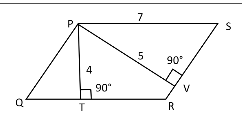
\includegraphics[width=0.7\columnwidth]{fig 1.png}
    \caption{}
    \label{fig:fig8}
\end{figure}
  \hfill (GATE BT 2015)

    \item A cube of side 3 units is formed using smaller cubes of side 1 unit. Find the proportion of the number of faces of the smaller cubes visible to those which are NOT visible.

    \begin{multicols}{4}
    \begin{enumerate}
        \item $1 : 4$  
        \item $1 : 3$  
        \item $1 : 2$  
        \item $2 : 3$  
    \end{enumerate}
    \end{multicols}             \hfill (GATE BT 2015)

    \item Humpty Dumpty sits on a wall every day while having lunch. The wall sometimes breaks. A person sitting on the wall falls if the wall breaks.  
    Which one of the statements below is logically valid and can be inferred?

    \begin{enumerate}
        \item Humpty Dumpty always falls while having lunch  
        \item Humpty Dumpty does not fall sometimes while having lunch  
        \item Humpty Dumpty never falls during dinner  
        \item When Humpty Dumpty does not sit on the wall, the wall does not break  
    \end{enumerate}
    \hfill (GATE BT 2015)

    \item Which one of the following complement proteins is the initiator of the membrane attack complex?
    \begin{multicols}{4}
    \begin{enumerate}
        \item C3a  
        \item C3b  
        \item C5a  
        \item C5b  
    \end{enumerate}
    \end{multicols}             \hfill (GATE BT 2015)

    \item Levinthal's paradox is related to:
    \begin{multicols}{2}
    \begin{enumerate}
        \item protein secretion  
        \item protein degradation  
        \item protein folding  
        \item protein trafficking  
    \end{enumerate}
    \end{multicols}             \hfill (GATE BT 2015)

    \item Which one of the following is a second generation genetically engineered crop?
    \begin{multicols}{2}
    \begin{enumerate}
        \item Bt brinjal  
        \item Roundup soybean  
        \item Golden rice  
        \item Bt rice  
    \end{enumerate}
    \end{multicols}             \hfill (GATE BT 2015)

    \item Based on the heavy chain, which one of the following antibodies has multiple subtypes?
    \begin{multicols}{4}
    \begin{enumerate}
        \item $I_gM$
        \item $I_gD$  
        \item $I_gE$  
        \item $I_gG$  
    \end{enumerate}
    \end{multicols}             \hfill (GATE BT 2015)

    \item The cytokinetic organelle in plant cells is:
    \begin{multicols}{4}
    \begin{enumerate}
        \item centriole  
        \item phragmoplast  
        \item proplastid  
        \item chromoplastid  
    \end{enumerate}
    \end{multicols}             \hfill (GATE BT 2015)


    \item Anergy refers to:
    \begin{multicols}{2}
    \begin{enumerate}
        \item mitochondrial dysfunction  
        \item allergy to environmental antigens  
        \item unresponsiveness to antigens  
        \item a state of no energy  
    \end{enumerate}
    \end{multicols}             \hfill (GATE BT 2015)

    \item ABO blood group antigens in humans are differentiated from each other on the basis of:
    \begin{multicols}{4}
    \begin{enumerate}
        \item sialic acid  
        \item lipids  
        \item spectrin  
        \item glycoproteins  
    \end{enumerate}
    \end{multicols}             \hfill (GATE BT 2015)

    \item Which one of the following organisms is used for the determination of phenol coefficient of a disinfectant?
    \begin{multicols}{2}
    \begin{enumerate}
        \item \textit{Salmonella typhi}  
        \item \textit{Escherichia coli}  
        \item \textit{Candida albicans}  
        \item \textit{Bacillus psychrophilus}  
    \end{enumerate}
    \end{multicols}             \hfill (GATE BT 2015)

    \item A single subunit enzyme converts 420 $\mu$mol of substrate to product in one minute. The activity of the enzyme is \underline{\hspace{2cm}} $\times 10^{-6}$ Katal.  
    \hfill(GATE BT 2015)

    \item Which one of the following amino acids has the highest probability to be found on the surface of a typical globular protein in aqueous environment?
    \begin{multicols}{4}
    \begin{enumerate}
        \item Ala  
        \item Val  
        \item Arg  
        \item Ile  
    \end{enumerate}
    \end{multicols}             \hfill (GATE BT 2015)

    \item Which one of the following is \textbf{NOT} a product of denitrification in \textit{Pseudomonas}?
    \begin{multicols}{4}
        \begin{enumerate}
            \item $N_{2}$
            \item $N_{2}O$
            \item $NO_{2}^{-}$
            \item $NH_{4}^{+}$
        \end{enumerate}
    \end{multicols}             \hfill (GATE BT 2015)

    %------------ Question 22 (NAT) -----------------
    \item The determinant of the matrix 
    $
    \begin{bmatrix}
    3 & 0 & 0 \\
    2 & 5 & 0 \\
    6 & -8 & -4
    \end{bmatrix}
    $
    is \_\_\_\_\_.
    \hfill (GATE BT 2015)

    %------------ Question 23 (MCQ) -----------------
    \item Which one of the following features is \textbf{NOT} required in a prokaryotic expression vector?
    \begin{multicols}{4}
        \begin{enumerate}
            \item $oriC$
            \item Selection marker
            \item CMV promoter
            \item Ribosome binding site
        \end{enumerate}
    \end{multicols}             \hfill (GATE BT 2015)

    %------------ Question 24 (MCQ) -----------------
    \item Production of monoclonal antibodies by hybridoma technology requires
    \begin{multicols}{4}
        \begin{enumerate}
            \item splenocytes
            \item osteocytes
            \item hepatocytes
            \item thymocytes
        \end{enumerate}
    \end{multicols}             \hfill (GATE BT 2015)

    %------------ Question 25 (MCQ) -----------------
    \item Which one of the following is \textbf{INCORRECT} about a typical apoptotic cell?
        \begin{enumerate}
            \item Phosphatidylserine is presented on the outer cell surface
            \item Cytochrome c is released from mitochondria
            \item Mitochondrial membrane potential does not change
            \item Annexin-V binds to the cell surface
        \end{enumerate}
         \hfill (GATE BT 2015)


    %------------ Question 26 (MCQ) -----------------
    \item Identify the file format given below:  

    \texttt{>P1; JMFD} \\
    \texttt{Protein X -- \textit{Homo sapiens}} \\
    \texttt{MKALTARQQEVFLDRDHISRTLRQQGDWL}

    \begin{multicols}{4}
        \begin{enumerate}
            \item GDE
            \item FASTA
            \item NBRF
            \item GCG
        \end{enumerate}
    \end{multicols}             \hfill (GATE BT 2015)

    %------------ Question 27 (MCQ) -----------------
    \item Which one of the following relations holds true for the specific growth rate ($\mu$) of a microorganism in the death phase?  

    \begin{multicols}{2}
        \begin{enumerate}
            \item $\mu = 0$
            \item $\mu < 0$
            \item $\mu = \mu_{\max}$
            \item $0 < \mu < \mu_{\max}$
        \end{enumerate}
    \end{multicols}             \hfill (GATE BT 2015)

    %------------ Question 28 (MCQ) -----------------
    \item How many 3-tuples are possible for the following amino acid sequence?  

    \texttt{MADCMWDISEASE}

    \begin{multicols}{4}
        \begin{enumerate}
            \item 4
            \item 5
            \item 11
            \item 12
        \end{enumerate}
    \end{multicols}             \hfill (GATE BT 2015)

    %------------ Question 29 (MCQ) -----------------
    \item How many different protein sequences of 100 residues can be generated using 20 standard amino acids?

    \begin{multicols}{4}
        \begin{enumerate}
            \item $100^{20}$
            \item $100 \times 20$
            \item $20^{100}$
            \item $100! \times 20!$
        \end{enumerate}
    \end{multicols}             \hfill (GATE BT 2015)


    %------------ Question 30 (MCQ) -----------------
    \item In DNA sequencing reactions using the chain termination method, the ratio of ddNTPs to dNTPs should be

    \begin{multicols}{2}
        \begin{enumerate}
            \item $0$
            \item $< 1$
            \item $1$
            \item $> 1$
        \end{enumerate}
    \end{multicols}             \hfill (GATE BT 2015)

    %------------ Question 31 (MCQ with Figure) -----------------
    \item Which one of the following graphs represents uncompetitive inhibition?

    \begin{multicols}{2}
        \begin{enumerate}
     \item \begin{figure}[H]
        \centering
        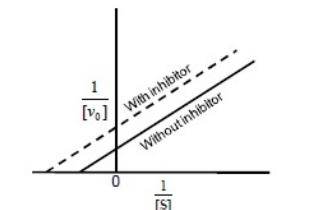
\includegraphics[width=0.8\columnwidth]{fig 2.png}
        \caption{}
        \label{fig:q31}
    \end{figure}
            \item \begin{figure}[H]
        \centering
        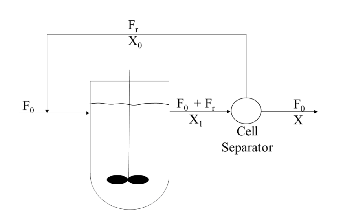
\includegraphics[width=0.8\columnwidth]{fig 3.png}
        \caption{}
        \label{fig:q31}
    \end{figure}
            \item \begin{figure}[H]
        \centering
        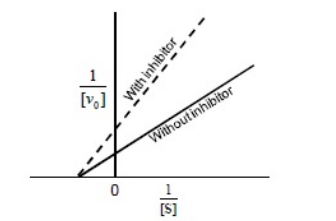
\includegraphics[width=0.8\columnwidth]{fig 4.png}
        \caption{}
        \label{fig:q31}
    \end{figure}
            \item \begin{figure}[H]
        \centering
        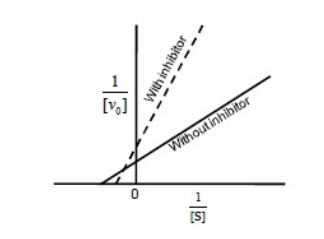
\includegraphics[width=0.8\columnwidth]{fig 5.png}
        \caption{}
        \label{fig:q31}
    \end{figure}
        \end{enumerate}
    \end{multicols}             \hfill (GATE BT 2015)


    %------------ Question 32 (MCQ with DNA sequence) -----------------
    \item Choose the appropriate pair of primers to amplify the following DNA fragment by the polymerase chain reaction (PCR):  

    $
    \begin{aligned}
    &5' - GACCTGTGG -------------------------- ATACGGGAT - 3' \\
    &3' - CTGGACACC -------------------------- TATGCCCTA - 5'
    \end{aligned}
    $

    Primers:  
    $
    \begin{aligned}
    \text{P. } & 5' - GACCTGTGG - 3' \\
    \text{Q. } & 5' - CCACAGGTC - 3' \\
    \text{R. } & 5' - TAGGGGATA - 3' \\
    \text{S. } & 5' - ATCCCGTAT - 3'
    \end{aligned}
    $

    \begin{multicols}{4}
        \begin{enumerate}
            \item P and R
            \item P and S
            \item Q and R
            \item Q and S
        \end{enumerate}
    \end{multicols}             \hfill (GATE BT 2015)

    %------------ Question 33 (NAT) -----------------
    \item Consider the following infinite series: 
    
\begin{center}
    $ 1 + r + r^2 + r^3 + \dots \infty $
\end{center}
    If $r = 0.3$, then the sum of this infinite series is \_\_\_\_\_\_\_.


    \item The system of linear equations in two variables shown below will have infinite solutions, if and only if, $b$ is equal to \_\_\_\_\_\_\_\_.

        \[
        2x_{1} + x_{2} = 3
        \]
        \[
        5x_{1} + bx_{2} = 7.5
        \]
         \hfill (GATE BT 2015)



% ---------- Question 35 (MCQ with figure) ----------
\item The interaction between an antigen (Ag) and a single-chain antibody (Ab) was studied using Scatchard analysis. The result is shown below.

\begin{figure}[H]
    \centering
    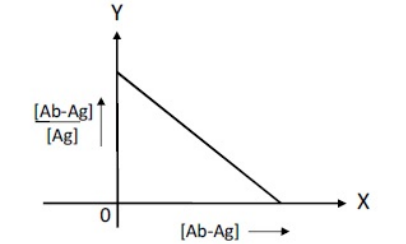
\includegraphics[width=0.5\linewidth]{fig 6.png}
    \caption{}
    \label{fig:scatchard}
\end{figure}

The affinity of interaction and the total concentration of antibody, respectively, can be determined from:

\begin{multicols}{2}
\begin{enumerate}
    \item slope and Y-intercept
    \item Y-intercept and slope
    \item X-intercept and slope
    \item slope and X-intercept
\end{enumerate}
\end{multicols} \hfill (GATE BT 2015)


% ---------- Question 36 (NAT with table) ----------
\item An isolated population on an island has the following genotypic frequencies:

\begin{table}[H]
    \centering
    \begin{tabular}{|c|c|c|c|}
    \hline
    Genotype & $AA$ & $Aa$ & $aa$ \\
    \hline
    Frequency & 0.3 & 0.4 & 0.3 \\
    \hline
    \end{tabular}
    \label{tab:genotype}
\end{table}

Assuming that there are only two alleles ($A$ and $a$) for the gene, the genotypic frequency of $AA$ in the next generation will be \_\_\_\_\_\_\_.
 \hfill (GATE BT 2015)

% ---------- Question 37 (MCQ without figure) ----------
\item How many rooted and unrooted phylogenetic trees, respectively, are possible with four different sequences?

\begin{multicols}{4}
\begin{enumerate}
    \item 3 and 15
    \item 15 and 3
    \item 15 and 12
    \item 12 and 3
\end{enumerate}
\end{multicols} \hfill (GATE BT 2015)


\item Match the compounds in \textbf{Group I} with the correct entries in \textbf{Group II}.  

\begin{table}[H]
\begin{tabular}{cc}
\textbf{Group I} & \textbf{Group II} \\
P) Cyanide          & 1) K$^{+}$ ionophore \\
Q) Antimycin A      & 2) Electron transfer from cytochrome $b$ to cytochrome $c_{1}$ \\
R) Valinomycin      & 3) F$_{1}$ subunit of ATP synthase \\
S) Aurovertin       & 4) Cytochrome oxidase \\
                    & 5) Adenine nucleotide translocase \\
\end{tabular}
\end{table}
\begin{multicols}{2}
\begin{enumerate}
    \item[(A)] P-5, Q-2, R-3, S-1
    \item[(B)] P-5, Q-2, R-1, S-3
    \item[(C)] P-4, Q-2, R-1, S-3
    \item[(D)] P-4, Q-5, R-3, S-1
\end{enumerate}
\end{multicols}\hfill (GATE BT 2015)

% ---------- Question 39 (MCQ Matrix) ----------
\item What are the eigenvalues of the following matrix?
\[
\begin{bmatrix}
1 & 1 \\
-2 & 4
\end{bmatrix}
\]

\begin{multicols}{4}
\begin{enumerate}
    \item 2 and 3
    \item -2 and 3
    \item 2 and -3
    \item -2 and -3
\end{enumerate}
\end{multicols}\hfill (GATE BT 2015)

% ---------- Question 40 (NAT) ----------
\item For a discrete random variable $X$, $ran(X)=\{0,1,2,3\}$ and the cumulative probability $F(X)$ is shown below:

\begin{table}[H]
\centering
\begin{tabular}{|c|c|c|c|c|}
\hline
$X$ & 0 & 1 & 2 & 3 \\
\hline
$F(X)$ & 0.5 & 0.6 & 0.8 & 1.0 \\
\hline
\end{tabular}
\end{table}

The mean value of $X$ is \_\_\_\_\_\_\_\_.
\hfill (GATE BT 2015)



% ---------- Question 41 (Matching type MCQ) ----------
\item Match the drugs in \textbf{Group I} with their mechanism of action in \textbf{Group II}.

\begin{table}[H]
\begin{tabular}{cc}
\textbf{Group I} & \textbf{Group II}  \\
P)  Paclitaxel      & 1)  Inhibits protein translation \\
Q)  Colchicine      & 2) Inhibits microtubule depolymerization \\
R)  Etoposide       & 3)  Inhibits DNA replication \\
S)  Methotrexate    & 4)  Alkylates DNA \\
              & 5) Inhibits dihydrofolate reductase \\
               & 6)  Inhibits microtubule polymerization \\

\end{tabular}
\end{table}

\begin{multicols}{2}
\begin{enumerate}
    \item P-1, Q-6, R-3, S-4
    \item P-2, Q-6, R-3, S-5
    \item P-1, Q-3, R-6, S-5
    \item P-2, Q-3, R-6, S-4
\end{enumerate}
\end{multicols}\hfill (GATE BT 2015)


% ---------- Question 42 (MCQ with math) ----------
\item The limit of the function $\left(1 + \tfrac{x}{n}\right)^{n}$ as $n \to \infty$ is

\begin{multicols}{2}
\begin{enumerate}
    \item $\ln x$
    \item $\ln \tfrac{1}{x}$
    \item $e^{x}$
    \item $e^{x}$ % duplicate for correct representation
\end{enumerate}
\end{multicols}\hfill (GATE BT 2015)


\item Match the cells in \textbf{Group I} with their corresponding entries in \textbf{Group II}.  

\begin{table}[H]
\begin{tabular}{cc}
\textbf{Group I} & \textbf{Group II} \\
P) Mast cells              & 1) Activation of the complement pathway \\
Q) Natural killer cells    & 2) Expression of CD56 \\
R) Neutrophils             & 3) Contains azurophilic granules \\
S) Dendritic cells         & 4) Defense against helminthic infection \\
                          & 5) Production of antibodies specific to bacteria \\
                          & 6) Contains long membranous projections \\
\end{tabular}
\end{table}

\begin{multicols}{2}
\begin{enumerate}
    \item P-4, Q-2, R-3, S-5
    \item P-4, Q-2, R-3, S-6
    \item P-3, Q-1, R-2, S-5
    \item P-3, Q-1, R-2, S-6
\end{enumerate}
\end{multicols}\hfill (GATE BT 2015)

\item Oxygen transfer was measured in a stirred tank bioreactor using dynamic method. The dissolved oxygen tension was found to be $80\%$ air saturation under steady state conditions. The measured oxygen tensions at $7 \, s$ and $17 \, s$ were $55\%$ and $68\%$ air saturation, respectively. The volumetric mass transfer coefficient $k_{L}a$ is \underline{\hspace{2cm}} $s^{-1}$.

\item Match the microorganisms in \textbf{Group I} with their fermentation products in \textbf{Group II}.  

\begin{table}[H]
\begin{tabular}{cc}
\textbf{Group I} & \textbf{Group II} \\
P) \textit{Leuconostoc mesenteroides}   & 1) Cobalamin \\
Q) \textit{Rhizopus oryzae}             & 2) Sorbose \\
R) \textit{Gluconobacter suboxydans}    & 3) Dextran \\
S) \textit{Streptomyces olivaceus}      & 4) Lactic acid \\
                                        & 5) Butanol \\
\end{tabular}
\end{table}

\begin{multicols}{2}
\begin{enumerate}
    \item P-5, Q-4, R-2, S-1
    \item P-5, Q-3, R-2, S-4
    \item P-3, Q-4, R-1, S-2
    \item P-3, Q-4, R-2, S-1
\end{enumerate}
\end{multicols}\hfill (GATE BT 2015)

\item Plasmid DNA ($0.5 \, \mu g$) containing an ampicillin resistance marker was added to $200 \, \mu l$ of competent cells. The transformed competent cells were diluted $10{,}000$ times, out of which $50 \, \mu l$ was plated on agar plates containing ampicillin. A total of $35$ colonies were obtained. The transformation efficiency is \underline{\hspace{2cm}} $\times 10^{6} \, \text{cfu} \cdot \mu g^{-1}$.
\hfill (GATE BT 2015)


\item Match the reagents in \textbf{Group I} with their preferred cleavage sites in \textbf{Group II}.  

\begin{table}[H]
\begin{tabular}{cc}
\textbf{Group I} & \textbf{Group II} \\
P) Cyanogen bromide                & 1) Carboxyl side of methionine \\
Q) o-Iodosobenzoate                & 2) Amino side of methionine \\
R) Hydroxylamine                   & 3) Carboxyl side of tryptophan \\
S) 2-Nitro-5-thiocyanobenzoate     & 4) Amino side of cysteine \\
                                   & 5) Asparagine-glycine bonds \\
\end{tabular}
\end{table}
\begin{multicols}{2}
\begin{enumerate}
    \item P-1, Q-3, R-5, S-4
    \item P-2, Q-3, R-1, S-4
    \item P-1, Q-2, R-5, S-4
    \item P-4, Q-2, R-5, S-3
\end{enumerate}
\end{multicols}\hfill (GATE BT 2015)

% ---------- Question 48 ----------



\item\textit{Saccharomyces cerevisiae} produces ethanol by fermentation. The theoretical yield of ethanol from $2.5 \, g$ of glucose is \underline{\hspace{2cm}} $g$.
\hfill (GATE BT 2015)


% ---------- Question 49 ----------


\item Choose the \textbf{CORRECT} sequence of steps involved in cytoplast production:

\begin{enumerate}
    \item Digestion of cell wall $\rightarrow$ protoplast viability $\rightarrow$ cybrid formation $\rightarrow$ osmotic stabilizer \\
    \item Osmotic stabilizer $\rightarrow$ digestion of cell wall $\rightarrow$ protoplast viability $\rightarrow$ cybrid formation \\
    \item Protoplast viability $\rightarrow$ osmotic stabilizer $\rightarrow$ digestion of cell wall $\rightarrow$ cybrid formation \\
    \item Osmotic stabilizer $\rightarrow$ digestion of cell wall $\rightarrow$ cybrid formation $\rightarrow$ protoplast viability \\
\end{enumerate} 
\hfill (GATE BT 2015)

\item Match the antibiotics in \textbf{Group I} with their modes of action in \textbf{Group II}.  

\begin{table}[H]
\begin{tabular}{cc}
\textbf{Group I} & \textbf{Group II} \\
P) Chloramphenicol      & 1) Inhibits protein synthesis by acting on 30S ribosomal subunit \\
Q) Rifampicin           & 2) Interferes with DNA replication by inhibiting DNA gyrase \\
R) Tetracycline         & 3) Inhibits protein synthesis by acting on 50S ribosomal subunit \\
S) Quinolone            & 4) Interferes with RNA polymerase activity \\
                        & 5) Inhibits $\beta$-lactamase activity \\
\end{tabular}
\end{table}

\begin{multicols}{2}
\begin{enumerate}
    \item P-1, Q-2, R-3, S-5
    \item P-3, Q-4, R-1, S-2
    \item P-3, Q-2, R-1, S-4
    \item] P-1, Q-4, R-3, S-2
\end{enumerate}
\end{multicols}\hfill (GATE BT 2015)






% ---------- Question 51 ----------
\item The diameters of a large and a small vessel are $1.62 \, m$ and $16.2 \, cm$, respectively. The vessels are geometrically similar and operated under similar volumetric agitated power input. The mixing time in the small vessel was found to be $15 \, s$. Determine the mixing time (in seconds) in the large vessel.  

\begin{multicols}{4}
\begin{enumerate}
    \item $15$  
    \item $30$  
    \item $61$  
    \item $122$  
\end{enumerate}
\end{multicols}\hfill (GATE BT 2015)




% ---------- Question 52 ----------
\item If $A = \begin{bmatrix} 4 & 2 \\ 1 & 3 \end{bmatrix}$, then $A^{2} + 3A$ will be  

\begin{multicols}{2}
\begin{enumerate}
    \item $\begin{bmatrix} 30 & 20 \\ 10 & 20 \end{bmatrix}$  
    \item $\begin{bmatrix} 28 & 10 \\ 4 & 18 \end{bmatrix}$  
    \item $\begin{bmatrix} 31 & 13 \\ 7 & 21 \end{bmatrix}$  
    \item $\begin{bmatrix} 20 & 10 \\ 5 & 15 \end{bmatrix}$  
\end{enumerate}
\end{multicols}\hfill (GATE BT 2015)


% ---------- Question 53 ----------
\item Consider the following multiple sequence alignment of four DNA sequences:  

\[
\begin{array}{cccc}
A & C & T & A \\
A & C & T & G \\
A & G & T & C \\
A & G & C & T \\
\end{array}
\]

Shannon’s entropy of the above alignment is \underline{\hspace{2cm}}.
\hfill (GATE BT 2015)



% ---------- Question 54 ----------
\item The $K_i$ of a novel competitive inhibitor designed against an enzyme is  $2.5 \, \mu M$. The enzyme was assayed in the absence or presence of the inhibitor ($5 \, \mu M$) under identical conditions. The $K_m$ in the presence of the inhibitor was found to be $30 \, \mu M$. The $K_m$ in the absence of the inhibitor is \underline{\hspace{2cm}} $\mu M$. 
\hfill (GATE BT 2015)



% ---------- Question 55 ----------
\item A heterozygous tall plant ($Tt$) was crossed with a homozygous dwarf plant ($tt$). The resultant seeds were collected. If five seeds are chosen at random, then the probability (in \%) that exactly two of these seeds will yield dwarf plants is \underline{\hspace{2cm}}.
\hfill (GATE BT 2015)


 

% ---------- Question 56 ----------
\item Assuming random distribution of nucleotides, the average number of fragments generated upon digestion of a circular DNA of size $4.3 \times 10^{5}$ bp with \textit{A\textsubscript{lu}I} (5$'$-AG$\downarrow$CT-3$'$) is \underline{\hspace{2cm}} $\times 10^{3}$.
\hfill (GATE BT 2015)


% ---------- Question 57 ----------
\item A synchronous culture containing $1.8 \times 10^{5}$ monkey kidney cells was seeded into three identical flasks. The doubling time of these cells is $24 \, h$. After $24 \, h$, the cells from all the three flasks were pooled and dispensed equally into each well of three $6$-well plates. The number of cells in each well will be \underline{\hspace{2cm}} $\times 10^{4}$. 
\hfill (GATE BT 2015)




% ---------- Question 58 ----------
\item An \textit{in vitro} translation system can synthesize peptides in all three reading frames of the RNA template. 
When 5$'$-UCUCUCUC---(UC)$_n$---UCUCUCUC-3$'$ was used as the template in this \textit{in vitro} translation system, the synthesized peptides contained 50\% each of serine and leucine. 
When 5$'$-CCUCCUCCU---(CCU)$_n$---CCUCCU-3$'$ was used as the template, the synthesized peptides contained 33.3\% each of serine, leucine, and proline. 
Deduce the codon for proline.  

\begin{multicols}{4}
\begin{enumerate}
\item UCU  
\item CUC  
\item CCU  
\item UCC  
\end{enumerate}
\end{multicols}\hfill (GATE BT 2015)



% ---------- Question 59 ----------
\item Three distinct antigens X, Y and Z were used to raise antibodies. Antigen Z was injected in a mouse on day zero followed by the administration of antigens X and Y on day 28. A second injection of antigen X was administered on day 70. The antibody titers were monitored in the serum every day and the results are shown below:

\begin{figure}[H]
\centering
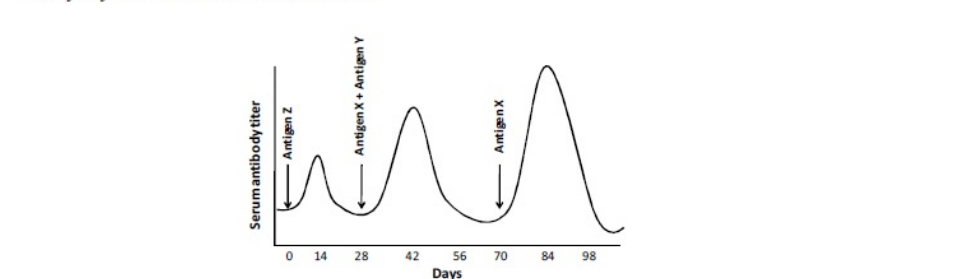
\includegraphics[width=0.7\columnwidth]{fig 7.png}
\caption{}
\label{fig:antibody}
\end{figure}

Which one of the following statements regarding the antibody titers in the serum is \textbf{INCORRECT}?  


\begin{enumerate}
\item Z-specific IgG will be high on day 14  
\item X-specific antibody titer will be high on day 84  
\item X-specific IgG will be high on day 42  
\item Y-specific IgG will be high on day 84  
\end{enumerate}\hfill (GATE BT 2015)

% ---------- Question 60 ----------
\item The standard free energy change ($\Delta G^{\circ\prime}$) for ATP hydrolysis is $-30 \, \text{kJ}\,\text{mol}^{-1}$. 
The \textit{in vivo} concentrations of ATP, ADP and P$_i$ in \textit{E.~coli} are $7.90$, $1.04$ and $7.90$ mM, respectively. 
When \textit{E.~coli} cells are cultured at $37^{\circ} \mathrm{C}$, the free energy change ($\Delta G$) for ATP hydrolysis \textit{in vivo} is \underline{\hspace{2cm}} kJ mol$^{-1}$. 
\hfill (GATE BT 2015)


% ---------- Question 61 ----------
\item In a fed-batch culture, $200 \, \text{g L}^{-1}$ glucose solution is added at a flow rate of $50 \, \text{L h}^{-1}$. 
The initial culture volume (at quasi steady state) and the initial cell concentration are $600 \, \text{L}$ and $20 \, \text{g L}^{-1}$, respectively. 
The yield coefficient ($Y_{x/s}$) is $0.5 \, \text{g cell mass g substrate}^{-1}$.  
The cell concentration ($\text{g L}^{-1}$) at quasi steady state at $t = 8 \, \text{h}$ is  

\begin{multicols}{4}
\begin{enumerate}
\item $40$  
\item $52$  
\item $60$  
\item $68$  
\end{enumerate}
\end{multicols}\hfill (GATE BT 2015)


% ---------- Question 62 ----------
\item Cytoplasmic extract from the wild type strain of a bacterium has the ability to convert a colorless substrate ($S$) to a colored product ($P$) via three colorless intermediates $X$, $Y$ and $Z$, in that order. Each step of the pathway involves a specific enzyme coded by a distinct gene. Four mutant strains ($a^-$, $b^-$, $c^-$, $d^-$) were isolated, whose extracts are incapable of producing the colored product in the presence of $S$. In a series of experiments, extracts from the individual mutants were incubated with $X$, $Y$, or $Z$ and scored for color development. The data are summarized in the table below. (Yes: color developed, No: no color developed)  

\begin{figure}[H]
\centering
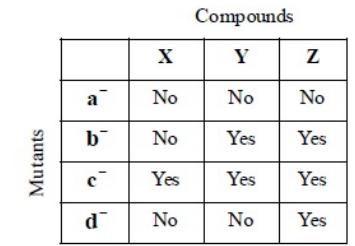
\includegraphics[width=0.7\columnwidth]{fig 13.png}
\caption{}
\label{fig:Q62}
\end{figure}

Based on the data, which one of the following is the correct order of enzymes involved in the pathway?  

\begin{multicols}{2}
\begin{enumerate}
\item $S \xrightarrow{a} X \xrightarrow{c} Y \xrightarrow{b} Z \xrightarrow{d} P$
\item $S \xrightarrow{a} X \xrightarrow{d} Y \xrightarrow{b} Z \xrightarrow{c} P$
\item $S \xrightarrow{X} Y \xrightarrow{c} Z \xrightarrow{d} P$
\item $S \xrightarrow{c} X \xrightarrow{b} Y \xrightarrow{d} Z \xrightarrow{a} P$
\end{enumerate}
\end{multicols}\hfill (GATE BT 2015)



% ---------- Question 63 ----------
\item Samples of bacterial culture taken at 5 PM and then the next day at 5 AM were found to have $10^4$ and $10^7$ cells mL$^{-1}$, respectively. Assuming that both the samples were taken during the log phase of cell growth, the generation time of this bacterium will be \_\_\_\_\_\_\_\_\_\_ h.
\hfill (GATE BT 2015)



% ---------- Question 64 ----------
\item Biomass is being produced in a continuous stirred tank bioreactor of 750 L capacity. The sterile feed containing $8 \, \text{g L}^{-1}$ glucose as substrate was fed at a flow rate of $150 \, \text{L h}^{-1}$. The microbial system follows Monod’s model with $\mu_m = 0.4 \, \text{h}^{-1}$, $K_s = 1.5 \, \text{g L}^{-1}$ and $Y_{x/s} = 0.5 \, \text{g cell mass g}^{-1}$ substrate. Determine the cell productivity ($\text{g L}^{-1}\text{h}^{-1}$) at steady state.  

\begin{multicols}{4}
\begin{enumerate}
\item$0.85$  
\item $0.65$
\item $0.45$  
\item $0.25$  
\end{enumerate}
\end{multicols}\hfill (GATE BT 2015)


% ---------- Question 65 ----------
\item A linear double stranded DNA of length 8 kbp has three restriction sites. Each of these can either be a \textit{BamHI} or a \textit{HaeIII} site. The DNA was digested completely with both enzymes. The products were purified and subjected to an end-filling reaction using the Klenow fragment and [$\alpha$-$^{32}$P]-dCTP. The products of the end-filling reaction were purified, resolved by electrophoresis, stained with ethidium bromide (EtBr) and then subjected to autoradiography. The corresponding images are shown below.

\begin{figure}[H]
    \centering
    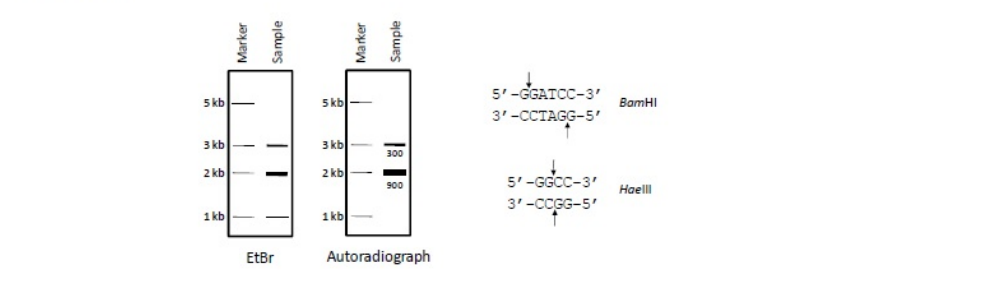
\includegraphics[width=0.7\columnwidth]{fig 8.png}
    \caption{}
    \label{fig:Q65}
\end{figure}

The numbers below each band in the sample lane in the autoradiograph represent their mean signal intensity in arbitrary units. Which one of the following options is the correct restriction map of the DNA?

\begin{multicols}{2}
\begin{enumerate}
\item \begin{figure}[H]
    \centering
    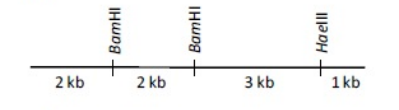
\includegraphics[width=0.7\columnwidth]{fig 9.png}
    \caption{}
    \label{fig9}
\end{figure}
\item \begin{figure}[H]
    \centering
    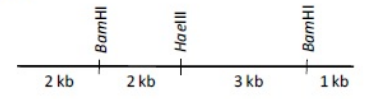
\includegraphics[width=0.7\columnwidth]{fig 10.png}
    \caption{}
    \label{fig10}
\end{figure}
\item \begin{figure}[H]
    \centering
    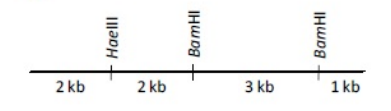
\includegraphics[width=0.7\columnwidth]{fig 11.png}
    \caption{}
    \label{fig:Q65}
\end{figure}
\item \begin{figure}[H]
    \centering
    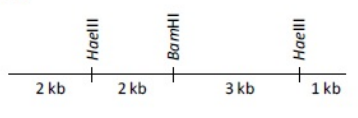
\includegraphics[width=0.7\columnwidth]{fig 12.png}
    \caption{}
    \label{fig:Q65}
\end{figure}
\end{enumerate}
\end{multicols}\hfill (GATE BT 2015)

\end{enumerate}
\end{document}